% ============================================================================
%  MCKL/manual/tex/core.tex
% ----------------------------------------------------------------------------
%  MCKL: Monte Carlo Kernel Library
% ----------------------------------------------------------------------------
%  Copyright (c) 2013-2016, Yan Zhou
%  All rights reserved.
%
%  Redistribution and use in source and binary forms, with or without
%  modification, are permitted provided that the following conditions are met:
%
%    Redistributions of source code must retain the above copyright notice,
%    this list of conditions and the following disclaimer.
%
%    Redistributions in binary form must reproduce the above copyright notice,
%    this list of conditions and the following disclaimer in the documentation
%    and/or other materials provided with the distribution.
%
%  THIS SOFTWARE IS PROVIDED BY THE COPYRIGHT HOLDERS AND CONTRIBUTORS "AS IS"
%  AND ANY EXPRESS OR IMPLIED WARRANTIES, INCLUDING, BUT NOT LIMITED TO, THE
%  IMPLIED WARRANTIES OF MERCHANTABILITY AND FITNESS FOR A PARTICULAR PURPOSE
%  ARE DISCLAIMED. IN NO EVENT SHALL THE COPYRIGHT HOLDER OR CONTRIBUTORS BE
%  LIABLE FOR ANY DIRECT, INDIRECT, INCIDENTAL, SPECIAL, EXEMPLARY, OR
%  CONSEQUENTIAL DAMAGES (INCLUDING, BUT NOT LIMITED TO, PROCUREMENT OF
%  SUBSTITUTE GOODS OR SERVICES; LOSS OF USE, DATA, OR PROFITS; OR BUSINESS
%  INTERRUPTION) HOWEVER CAUSED AND ON ANY THEORY OF LIABILITY, WHETHER IN
%  CONTRACT, STRICT LIABILITY, OR TORT (INCLUDING NEGLIGENCE OR OTHERWISE)
%  ARISING IN ANY WAY OUT OF THE USE OF THIS SOFTWARE, EVEN IF ADVISED OF THE
%  POSSIBILITY OF SUCH DAMAGE.
% ============================================================================

\chapter{Core concepts}
\label{chap:Core concepts}

In this chapter, we introduce the core concepts of the library. There are five
of them. At the center is a user defined class that represents the state space.
It shall contain the state values $X_{1:N_t}^t$. This class may also contain
other members that is specific for the model, such as its data set. Next are
the weights $W_{1:N_t}^t$. These two form the particle system $S_{1:N_t}^t$,
where $S_i^t = (X_i^t,W_i^t)$. A sampler operates on a particle system to
produce samples iteratively. A sampler might also use some monitors to
calculate some estimates $\varphi^t(S_{1:N_t}^t)$ as it progresses. These
concepts are all abstracted in the library. For brevity, in the following we
will drop the time dependent index $t$.

\section{State}
\label{sec:State}

Let $E$ be the state space. A state object represents the states $X_{1:N}$ and
everything it depends on. If there exists an integer $d\ge1$ and some space
$\calX$ such that $E\subseteq\calX^d$. Then, we can represent the states as an
$N$ by $d$ matrix. The element at row $i$ and column $j$ is thus the $j$\ith
component of $X_i$. The library provides a class template to abstract this type
of state space,
\begin{Verbatim}
  template <MatrixLayout Layout, size_t Dim, typename ValueType>
  class StateMatrix;
\end{Verbatim}
where \verb|Layout| is either \verb|RowMajor| or \verb|ColMajor|, which
specifies the matrix layout, \verb|Dim| is the dimension of $X$, i.e., $d$ and
\verb|ValueType| represents values in $\calX$. For example, if
$E\subseteq\Real^d$, then one can use the following class,
\begin{Verbatim}
  StateMatrix<RowMajor, d, double> state(N);
\end{Verbatim}
This is not a general purpose matrix class for use such as linear algebra. It
is more of a container with a few additional methods. Below is some common
operations can be done on \verb|state|,
\begin{Verbatim}
  state.size();     // Get sample size
  state.dim();      // Get dimension
  state.row_size(); // Same as size()
  state.col_size(); // Same as dim()
  state.resize(N);  // Set sample size
  state(i, j);      // The element at row i, column j
  state.at(i, j);   // Same as above but with assertion
\end{Verbatim}
If the template parameter \verb|Dim| is equal to zero, then it is assumed that
the dimension is dynamic and may change later. In this case, there is an
additional constructor and other methods,
\begin{Verbatim}
  StateMatrix<RowMajor, Dynamic, double> state(N, d);
  state.resize(N, d);  // Set sample size and dimension
  state.resize_dim(d); // Set dimension
\end{Verbatim}
The enumerator \verb|Dynamic| above has the value zero. Note that, these
methods are only available when the template parameter \verb|Dim| is zero.
Attempting to call these methods when it is positive will result in
compile-time errors. Let $p$ be the minimum of the original and new sample
sizes, and $q$ be the minimum of the original and new dimensions. All the
methods that change the size of the matrix will preserve the $p$ by $q$ matrix
at the upper left corner of the original. It is also possible to get pointers
to the raw data,
\begin{Verbatim}
  state.data();       // &state(0, 0)
  state.row_data(i);  // &state(i, 0)
  state.col_data(i);  // &state(0, j)
  state.row_stride(); // &state(i, j + 1) - &state(i, j)
  state.col_stride(); // &state(i + 1, j) - &state(i, j)
\end{Verbatim}
These pointers can provide either read only or read and write access to the raw
data, depends on whether or not the \verb|state| object is constant. Note that,
the strides of the pointers returned by \verb|row_data| and \verb|col_data|
depends on the template parameter \verb|Layout|. To iterate over a specific
row,
\begin{Verbatim}
  auto rowptr = state.row_data(i);
  auto stride = state.row_stride();
  auto d = state.dim();
  for (size_type j = 0; j != d; ++j, rowptr += stride)
      /* *rowptr is the as state(i, j) */;
\end{Verbatim}
And similarly, to iterate over a specific column,
\begin{Verbatim}
  auto colptr = state.col_data(j);
  auto stride = state.col_stride();
  auto n = state.size();
  for (size_type i = 0; i != n; ++i, colptr += stride)
      /* *colptr is the as state(i, j) */;
\end{Verbatim}
One can also retrieve a whole row or column through an output iterator. For
example, to read the rows~1 and~3 into a vector,
\begin{Verbatim}
  std::vector<ValueType> row13(state.dim() * 2);
  auto first = row13.begin();
  first = state.read_row(1, first);
  first = state.read_row(3, first);
\end{Verbatim}
And similarly, to read columns~2 and~4 into a vector,
\begin{Verbatim}
  std::vector<ValueType> col24(state.size() * 2);
  auto first = col24.begin();
  first = state.read_col(2, first);
  first = state.read_col(4, first);
\end{Verbatim}
The methods \verb|read_row| and \verb|read_col| return output iterators that
point to one pass the last element in the destination range, similar to that of
\verb|std::copy|, etc. To read the whole matrix into a vector,
\begin{Verbatim}
  std::vector<ValueType> mat(state.size() * state.dim());
  state.read(RowMajor, mat.begin());
\end{Verbatim}
The first parameter is matrix layout of the output matrix. There are two more
methods, whose purpose will become clear later. The first is,
\begin{Verbatim}
  void duplicate(size_type src, size_type dst);
\end{Verbatim}
Let the value of \verb|src| and \verb|dst| be $p$ and $q$, respectively. This
method sets $X^q = X^p$. In other words, $X^p$ is duplicated while $X^q$ is
eliminated. The other method is,
\begin{Verbatim}
  template <typename IntType, typename InputIter>
  void select(IntType N, InputIter index);
\end{Verbatim}
The first argument is the new sample size, say $\hat{N}$ and \verb|index| is an
$\hat{N}$-vector, say $a_{1:\hat{N}}$. This method selects samples to form a
new collection $\hat{X}_{1:\hat{N}}$  by setting $\hat{X}_i = X_{a_i}$ for $i =
1,\dots,\hat{N}$. The new sample size $\hat{N}$ does not have to be the same as
the original, say $N$. This is closely related to the selection step of \smc
algorithms. Let $r_i = \sum_{j = 1}^{\hat{N}}\bbI_{\{i\}}(a_j)$. Then it is
required that $a_i = i$ for all $r_i > 0$, $i = 1,\dots,\min\{N, \hat{N}\}$.

\section{Weight}
\label{sec:Weight}

The weights $W_{1:N}$ is abstracted by the class \verb|Weight|. For example,
\begin{Verbatim}
  Weight w(N);
  w.size();    // Get sample size
  w.resize(N); // Set sample size
\end{Verbatim}
One important property of \verb|Weight| is that, $W_{1:N}$ is always
normalized such that $\sum_{i=1}^N W_i = 1$. For example, after the
construction or resizing, the weights are set to be equal, i.e., $W_i = 1 / N$,
for $i = 1,\dots,N$. This can also be done manually,
\begin{Verbatim}
  w.set_equal();
\end{Verbatim}
The weights can be manipulated in various ways. Let \verb|v| be an input
iterator pointing to an $N$-vector $v_{1:N}$. To set $W_i \propto v_i$,
\begin{Verbatim}
  w.set(v);
\end{Verbatim}
To set $ W_i \propto W_i\EE^{v_i}$,
\begin{Verbatim}
  w.set_log(v);
\end{Verbatim}
To set weights incrementally, use
\begin{Verbatim}
  w.mul(v);
  w.add_log(v);
\end{Verbatim}
which set $W_i \propto W_iv_i$ and $W_i \propto W_i \EE^{v_i}$, respectively.
The value of \ess of the weights can be obtained by,
\begin{Verbatim}
  w.ess();
\end{Verbatim}
One may also draw an integer $0 \le k < N$ according to the weights by,
\begin{Verbatim}
  w.draw(rng);
\end{Verbatim}
where \verb|rng| is a \rng engine object. Last, one can obtain a pointer to the
raw data,
\begin{Verbatim}
  w.data();
\end{Verbatim}
or read all the weights into an output iterator,
\begin{Verbatim}
  w.read(first);
\end{Verbatim}
Unlike \verb|StateMatrix|, the pointer returned by the \verb|data| method
always provides read only access. In other words, \verb|Weight| does not
provide any means for user to change an individual $W_i$ without changing the
others. Conceptually, it is the relative weights that matter. And changing one
of them is in fact changing $W_{1:N}$ as a whole.

\section{Particle}
\label{sec:Particle}

A particle system, abstracted by the class template,
\begin{Verbatim}
  template <typename T>
  class Particle;
\end{Verbatim}
is formed by three parts. The first is an object of type \verb|T|, that
abstracts the states $X_{1:N}$. The second is a type \verb|Weight| object that
abstracts the weights $W_{1:N}$. And the third is a collection of \rng engines.
There are some restrictions on the type \verb|T|. The constructor of
\verb|Particle| is as the following,
\begin{Verbatim}
  template <typename... Args>
  explicit Particle(size_type N, Args &&... args)
\end{Verbatim}
The first argument is the sample size. This and all other arguments, are passed
down to the constructor of type \verb|T|. For example,
\begin{Verbatim}
  using T = StateMatrix<RowMajor, Dynamic, double>;
  Particle<T> particle(N, d);
\end{Verbatim}
will construct the \verb|StateMatrix| object with arguments \verb|N| and
\verb|d|. Therefore, \verb|T| must has a constructor that accepts an integer
value as its first argument. The additional acceptable arguments of the
constructor of \verb|Particle| is the same as those of \verb|T|. Second,
\verb|T| has to provide a \verb|select| method similar to that of
\verb|StateMatrix|. The library does not impose any restriction on the internal
structure of \verb|T|. And thus it cannot perform the selection by itself.
However, for more complicated situations, one can always define a class, say
\verb|ValueType| to represent the space $E$, and use a one dimension
\verb|StateMatrix| as the type \verb|T|. For example,
\begin{Verbatim}
  class ValueType; // User defined type
  using T = StateMatrix<RowMajor, 1, ValueType>;
  Particle<T> particle(N);
\end{Verbatim}
More usefully, one can create a new type by deriving from \verb|StateMatrix|.
Note that, though the \verb|select| method of \verb|StateMatrix| is written as
a function template that can accept any integers and input iterators as its
arguments, the user defined type \verb|T| only needs to support the following
signature,
\begin{Verbatim}
  ReturnType select(size_type N, const size_type *index);
\end{Verbatim}
where \verb|size_type| is \verb|T::size_type| if such a type exists, and
\verb|size_t| otherwise.

The \verb|Weight| type object is constructed with a single argument, the sample
size $N$. To retrieve references to the type \verb|T| and \verb|Weight|
objects, one can call,
\begin{Verbatim}
  particle.state();
  particle.weight();
\end{Verbatim}
respectively. Last but not least, the \verb|Particle| class also contains a
collection of \rng engines. The method,
\begin{Verbatim}
  particle.rng(i);
\end{Verbatim}
returns a reference to an \rng engine, specific to the $i$\ith particle. For $i
\ne j$, if the following,
\begin{Verbatim}
  auto &rng_i = particle.rng(i);
  auto &rng_j = particle.rng(j);
\end{Verbatim}
are called from two different threads, then \verb|rng_i| and \verb|rng_j| will
be instances of two independent \rng engines. The details are in
Section~\ref{sec:Multiple RNG streams}. The \verb|Particle| class also contains
an \rng engine independent of any particle,
\begin{Verbatim}
  auto &rng = particle.rng();
\end{Verbatim}

\subsection{Resize the particle system}
\label{sub:Resize the particle system}

The sample size of a particle system can be obtained by,
\begin{Verbatim}
  particle.size();
\end{Verbatim}
It can be changed. However, in Monte Carlo algorithms, one does not change the
sample size arbitrarily. Which samples to be preserved and possibly duplicated
and which samples to be eliminated, has to be done according to some algorithms
that produce desirable effects. There are a few methods to resize a particle
system. They share two common properties. They take the new sample size, say
$M$, as their first argument. The other is that in the end, they call the
\verb|select| method on the type \verb|T| object, with $M$ and an input
iterator, say \verb|index|, that points to an $M$-vector $a_{1:M}$ as
arguments. In addition they all call the \verb|resize| method on the type
\verb|Weight| object with $M$ as the argument. How the type \verb|T| handles
the call to the \verb|select| method is up to the user. But usually it should
behave similarly to that of \verb|StateMatrix|. Below is descriptions of each
method for resizing a particle system. They differ in how they generate the
index vector $a_{1:M}$. We will let $N$ denote the original sample size. Also,
for clarity, in the mathematical description of the vectors, we are using
indices starting with $1$, while in the actual program, the indices starts with
zero, as usual.

\subsubsection{Resize with given index vectors}

\begin{Verbatim}
  template <typename InputIter>
  void resize_by_index(size_type M, InputIter index);
\end{Verbatim}
This method takes the index vector as its input and passes it directly to the
\verb|select| method of \verb|T|.

\subsubsection{Resize with resampling algorithms}

\begin{Verbatim}
  template <typename ResampleType>
  void resize_by_resample(size_type M, ResampleType &&res)
\end{Verbatim}
This method generates the index vector according to a resampling algorithm. A
resampling algorithm produce the number of replications of each particle in the
original system. The function \verb|res| shall accept a call as the following,
\begin{Verbatim}
  res(N, M, rng, w, r);
\end{Verbatim}
where $N$ and $M$ are the original and new sample size, \verb|rng| is a
reference to an \rng engine, \verb|w| is a pointer of type \verb|double|, that
points to the $N$-vector of normalized weights. And last, \verb|r| is a pointer
of type \verb|size_type| that points to the $N$-vector of the number of
duplicates of each particles $r_{1:N}$. It is required that, the results shall
satisfy $r_i\ge0$ for $i=1,\dots,N$ and $\sum_{i=1}^N r_i = M$. The index
vector is generated such that,
\begin{gather*}
  a_i = i \text{ if } r_i > 0 \text{ for } i = 1,\dots,\min\{N, M\} \\
  \sum_{i=1}^M\bbI_{\{j\}}(a_i) = r_j \text{ for } j = 1,\dots,N
\end{gather*}

\subsubsection{Resize with uniform selection}

\begin{Verbatim}
  void resize_by_uniform(size_type M);
\end{Verbatim}
The index vector is generated such that, $\Prob(a_i = j) = 1/M$, for $i =
1,\dots,M$, $j = 1,\dots,N$. This is equivalent to Multinomial resampling with
equal weights.

\subsection{Clone the particle system}
\label{sub:Clone the particle system}

The \verb|Particle<T>| class has the usual special members, such as the copy
constructor, assignment operator, etc. They work just as usual. For example,
\begin{Verbatim}
  auto new_particle = particle;
\end{Verbatim}
This creates a new particle system as an exact duplicate of the original.
However, this ``exactness'' is often undesired. The duplicated particle system
will have exactly the same states of \rng engines as the original. And
therefore, any random samples generated from this new system will be exactly
the same as the original. This is hardly the desired effects in algorithms
where duplicating a particle system into multiple copies is required. In this
situation, one can use the \verb|clone| method,
\begin{Verbatim}
  auto new_particle = particle.clone();
\end{Verbatim}
In contrast to the copy constructor, this will create a new particle system
exactly the same as the original, except that all \rng engines within the new
system is re-seeded.

\subsection{Iterate the particle system}
\label{sub:Iterate the particle system}

As mentioned before, the library does not impose restrictions on how the states
shall be structured or accessed. Therefore it is not possible to access $X_i$
using methods of \verb|Particle|. Instead, one has to use methods of \verb|T|,
the type of the template parameter. For example,
\begin{Verbatim}
  using T = StateMatrix<RowMajor, d, double>;
  Particle<T> particle(N);
  particle.state()(i, j);
  particle.state().dim();
\end{Verbatim}
This is rather cumbersome and somehow too limited. The library provides a class
template,
\begin{Verbatim}
  template <typename T>
  class ParticleIndex;
\end{Verbatim}
that represents the index of particles within the system. It is constructed by
the index of the particle and a pointer to the particle system that it belongs
to. For example,
\begin{Verbatim}
  ParticleIndex<T> idx(i, &particle);
\end{Verbatim}
or alternatively,
\begin{Verbatim}
  auto idx = particle.index(i);
\end{Verbatim}
To access the particle system, use
\begin{Verbatim}
  idx.particle();     // A reference to particle
  idx.particle_ptr(); // A pointer to particle
\end{Verbatim}
For any type \verb|T|, the type \verb|ParticleIndex<T>| has the following
methods,
\begin{Verbatim}
  idx.i();   // The index used to construct idx, i
  idx.rng(); // => particle.rng(i);
\end{Verbatim}
If \verb|T| is a derived class of \verb|StateMatrix|, then
\begin{Verbatim}
  idx.dim();    // => particle.state().dim();
  idx.stride(); // => particle.state().row_stride();
  idx.data();   // => particle.state().row_data(i);
  idx(j);       // => particle.state()(i, j);
  idx.at(j);    // => particle.state().at(i, j);
\end{Verbatim}
That is, \verb|ParticleIndex| has an interface that depends on the type
\verb|T|. One can extend its interface by defining a special member class
template inside \verb|T|. For example,
\begin{Verbatim}
  using Base = StateMatrix<RowMajor, d, double>;

  class T : public Base
  {
      public:
      template <typename S>
      using idx_base = Base::particle_index_type<S>;

      template <typename S>
      class particle_index_type : public idx_base<S>
      {
          public:
          particle_index_type(
              size_type i, Particle<S> *pptr) :
              idx_base<S>(i, pptr)
          {
          }
      };
  };
\end{Verbatim}
The class \verb|ParticleIndex<T>| derives from \verb|T::particle_index_type<T>|
if such a member type exists. Otherwise, it has methods as described earlier
for any type \verb|T|. Therefore, it is possible to give it methods that are
more convenient for a particular problem. We will see examples later in
Section~\ref{sec:Example (PF)}.

The \verb|ParticleIndex| type can also be used like an random access iterator.
For example,
\begin{Verbatim}
  auto idx = particle(i);
  auto jdx = particle(j);
  ++idx;      // => particle.index(i + 1);
  idx--;      // => particle.index(i - 1);
  idx + n;    // => particle.index(i + n);
  idx - jdx;  // => i - j;
  idx == jdx; // => i == j;
\end{Verbatim}
Other comparison operators such as \verb|!=|, \verb|<|, etc., are also
defined. Note that, comparing or subtracting two indices from two different
particles systems is meaningless. This will result in runtime errors unless
debugging is disabled (see Section~\appref{sec:Error handling}). The increment
and decrement operators follow usual prefix and postfix semantics. However, it
is important to note that, \verb|ParticleIndex| \emph{is not} an iterator even
though it shares many common methods. Recall that, \verb|Particle| does not
have methods to access $X_i$ directly. And therefore it is not possible to
dereference a \verb|ParticleIndex| object to get a reference to $X_i$. Instead,
dereferencing an \verb|ParticleIndex| object will return a reference to itself.
This is similar for the member access operator and the index operator. For
example,
\begin{Verbatim}
  *idx;       // => idx
  idx->rng(); // => idx.rng();
  idx[n];     // => idx + n
\end{Verbatim}
These methods may at first seem pointless. However, it makes it possible to
iterate a \verb|Particle| object. For example,
\begin{Verbatim}
  for (auto idx : particle) {
      idx(0) = /* initialize the first dimension */;
      idx(1) = /* initialize the second dimension */;
      // ...
  }
\end{Verbatim}
This is equivalent to
\begin{Verbatim}
  for (size_t i = 0; i != particle.size(); ++i) {
      auto idx = particle.index(i);
      // ...
  }
\end{Verbatim}
More importantly, it allows the use of \verb|Particle| with algorithms. For
example,
\begin{Verbatim}
  auto s = std::accumulate(
      particle.begin(), particle.end(), 0.0,
      [](double s, ParticleIndex<T> idx) {
          return s + idx(0);
      });
\end{Verbatim}

\section{Monitor}
\label{sec:Monitor}

Let $\varphi(S_{1:N})$ be some estimator with values in $\Real^d$. It is often
of interest to monitor its value as the algorithm progresses. In the library,
this is done through the class template \verb|Monitor|. It has the following
constructor,
\begin{Verbatim}
  Monitor(
      size_t dim,
      const eval_type &eval,
      bool record_only = false,
      MonitorStage stage = MonitorMCMC);
\end{Verbatim}
The first parameter \verb|dim| is the dimension of $\varphi$, $d$. The second
is a user defined callback function. More specifically,
\begin{Verbatim}
  using eval_type = std::function<void(
      size_t, size_t, Particle<T> &, double *)>;
\end{Verbatim}
For example,
\begin{Verbatim}
  void phi(size_t t, size_t d, Particle<T> &particle, double *r);
\end{Verbatim}
When this function is called. The first argument passed to it is $t$, the
iteration number. The second is $d$, the dimension. The third is a reference to
the particle system at iteration $t$. And the last is a pointer to a vector for
output. The third parameter of the constructor, \verb|record_only|, determines
how shall the function above behave. If it is true, then the function
\verb|phi| shall return the value of $\varphi$ directly, and the output
parameter \verb|r| points to a $d$-vector. In this case, \verb|Monitor| merely
records the values of $\varphi$ at each iteration. On the other hand, if
\verb|record_only| is false, then it is assumed that $\varphi$ takes the
following form,
\begin{equation*}
  \varphi(X_{1:N}) = \sum_{i=1}^N W_i \varphi_i(X_i).
\end{equation*}
And the output parameter \verb|r| is an $N$ by $d$ row major matrix, with the
$d$-vector value $\varphi_i(X_i)$ written into each row of this matrix. And
each time \verb|phi| is called, \verb|Monitor| will compute and store the
result of the summation above. The last parameter of the constructor of
\verb|Monitor| specifies when shall the calculation of $\varphi$ be carried
out. We will defer its discussion until we introduce the sampler in the next
section. The evaluation object can be replaced later by the following method,
\begin{Verbatim}
  void eval(
      const eval_type &e,
      bool record_only = false,
      MonitorStage stage = MonitorMCMC);
\end{Verbatim}
One can retrieve the results in various ways. Every time a monitor being
evaluated, it records two values. The first is the iteration number $t$, at
which it was evaluated. The other is the value of $\varphi$. One can retrieve
these values using the following methods,
\begin{Verbatim}
  mon.iter_size();  // Total number of evaluations
  mon.index(j);     // Iteration number of the j-th evaluation
  mon.record(i, j); // The value of the i-th component
                    // of the result at the j-th evaluation
\end{Verbatim}
Note that, the monitor does not have to be added to a sampler before it
starting initialization. It can also be removed before the sampler finishing
all iterations. Therefore, the iteration numbers of a monitor being evaluated
are not necessarily the sequence $0,1,\dots,n$, where $n$ is the total number
of iterations.

\section{Sampler}
\label{sec:Sampler}

A sampler is formed by the particle system together with all the operations on
it. It is abstracted by the class template,
\begin{Verbatim}
  template <typename T>
  class Sampler;
\end{Verbatim}
The template parameter \verb|T| is the same as that of \verb|Particle|. Its
constructor takes arbitrary arguments,
\begin{Verbatim}
  template <typename... Args>
  explicit Sampler(Args &&... args)
\end{Verbatim}
and all arguments are passed down to the constructor of \verb|Particle|. For
example,
\begin{Verbatim}
  using T = StateMatrix<RowMajor, Dynamic, double>;
  Sampler<T> sampler(N, d);
\end{Verbatim}
Any callable objects that is convertible to the following can be used as
operations on the particle system,
\begin{Verbatim}
  using eval_type = std::function<void(size_t, Particle<T> &)>;
\end{Verbatim}
For example,
\begin{Verbatim}
  void eval(size_t iter, Particle<T> &particle);
\end{Verbatim}
Conceptually, such a function implement an operator $M(S_{1:N})$ such that a
new particle system $\hat{S}_{1:\hat{N}}$ is produced given the iteration
number $t$ and the original. It it often possible to decompose the operator $M$
into multiple simpler ones. And thus a sampler can have a sequence of
evaluation objects. Each of these evaluation objects can be added to the
sampler by the \verb|eval| method,
\begin{Verbatim}
  Sampler<T> &eval(const eval_type &e, SamplerStage stage);
\end{Verbatim}
For example,
\begin{Verbatim}
  sampler.eval(eval, SamplerInit | SamplerMove, true);
\end{Verbatim}
The first argument is the evaluation object. The sampler maintains a sequence
of evaluation steps. The new evaluation object will be appended to the existing
sequence. Note that, the order at which these objects being evaluated is the
same as the one they are added to the sampler. One can clear the sequence by,
\begin{Verbatim}
  sampler.eval_clear();
\end{Verbatim}
The second argument will be explained in the next section. The sampler can also
have an optional resampling step. This can be added to the sampler by the
following method,
\begin{Verbatim}
  Sampler<T> &resample_method(
      ResampleScheme scheme,
      double threshold = resample_threshold_always());
\end{Verbatim}
which uses a builtin resampling scheme of the library (see
Section~\ref{sec:Algorithm}). Or alternatively,
\begin{Verbatim}
  Sampler<T> &resample_method(
      const eval_type &res_eval,
      double threshold = resample_threshold_always());
\end{Verbatim}
In either case, the parameter \verb|threshold| specifies the condition under
which the resampling step will be actually performed. Let its value be
$\alpha$, resampling is performed if and only if $\ess < \alpha N$.

Multiple monitors can be added to a sampler. For example,
\begin{Verbatim}
  Monitor<T> mon(d, phi, false, MonitorMCMC);
  sampler.monitor("name", mon);
\end{Verbatim}
A reference to the named monitor can be retrieved,
\begin{Verbatim}
  auto &m = sampler.monitor("name");
\end{Verbatim}

\subsection{Initialization and iteration}
\label{sub:Initialization and iteration}

The sampler can be initialized,
\begin{Verbatim}
  sampler.initialize();
\end{Verbatim}
This will perform a few things. First, any record of previous operations on the
sampler will be cleared. The iteration number $t$ will be set to zero. And
then, there are three evaluation stages and three monitoring stages. They are
performed in the following order:

\begin{enumerate}
  \item \verb|SamplerInit|
  \item \verb|MonitorMove|
  \item Resample if $\ess < \alpha N$
  \item \verb|MonitorResample|
  \item \verb|SamplerMCMC|
  \item \verb|MonitorMCMC|
\end{enumerate}

Each evaluation object, added to the sampler through,
\begin{Verbatim}
  Sampler<T> &eval(const eval_type &e, SamplerStage stage);
\end{Verbatim}
will be evaluated at the \verb|SamplerInit|, etc., steps if the corresponding
stage is set (e.g., \verb|stage & SamplerInit| is non-zero). Similarly, every
monitor, constructed by,
\begin{Verbatim}
  Monitor(
      size_t dim,
      const eval_type &eval,
      bool record_only = false,
      MonitorStage stage = MonitorMCMC);
\end{Verbatim}
will be evaluated if the corresponding stage is the same (e.g., \verb|stage|
\emph{equal} to \verb|MonitorMove|). The sampler can be iterated,
\begin{Verbatim}
  sampler.iterate();  // iterate once
  sampler.iterate(n); // iterate n times
\end{Verbatim}
At each iteration, the steps performed is the same as initialization, except
that \verb|SamplerInit| is replaced by \verb|SamplerMove|. Therefore, one can
distinguish between operations for initialization or iteration only, and those
for every step. We will see an example in the next section.

\section{Example}
\label{sec:Example (PF)}

This is an example used in \cite{Johansen:2009wd}. Through this example, we
will show how to implement a simple particle filter. It shall walk one through
the basic features of the library introduced above.

\subsection{Model and algorithm}
\label{sub:Model and algorithm}

The state space model, known as the almost constant velocity model in the
tracking literature, provides a simple scenario. The state vector,
\begin{equation*}
  X^t = (\xpos^t, \ypos^t, \xvel^t, \yvel^t)^{\transpose}
\end{equation*}
contains the position and velocity of an object moving in a plane. Imperfect
observations $Y^t = (\xobs^t, \yobs^t)^{\transpose}$ of the positions are
possible at each time instance. The state and observation equations are linear
with additive noises,
\begin{align*}
  X^t &= AX^{t-1} + U^t \\
  Y^t &= BX^t + \delta V^t
\end{align*}
where
\begin{equation*}
  A = \begin{pmatrix}
    1 & 0 & \Delta & 0      \\
    0 & 1 & 0      & \Delta \\
    0 & 0 & 1      & 0      \\
    0 & 0 & 0      & 1
  \end{pmatrix} \qquad
  B = \begin{pmatrix}
    1 & 0 & 0 & 0 \\
    0 & 1 & 0 & 0 \\
  \end{pmatrix} \qquad
  \delta = 0.1
\end{equation*}
and we assume that the elements of the noise vector $U_t$ are independent
Gaussian with variance $0.02$ and $0.001$ for position and velocity,
respectively. The observation noise, $V_t$ comprises i.i.d.\ $t$-distributed
random variables with degree of freedom $\nu = 10$. The prior at time $0$
corresponds to an axis-aligned Gaussian with variance $4$ for the position
coordinates and $1$ for the velocity coordinates. The particle filter algorithm
is shown in Algorithm~\ref{alg:pf}.

\begin{algorithm}[t]
  \begin{algorithmic}
    \tophrule
    \STATE \COMMENT{Initialization}
    \STATE Set $t\leftarrow0$.
    \STATE Sample $\xpos^{0,i},\ypos^{0,i}\sim\calN(0,4)$ and
    $\xvel^{0,i},\yvel^{0,i}\sim\calN(0,1)$.
    \STATE Weight $W_i^0 \propto \exp\{\ell(X_i^0|Y_0)\}$

    \REPEAT
    \STATE \COMMENT{Iteration}
    \STATE Set $t\leftarrow t + 1$.
    \STATE Sample
    \begin{align*}
      \xpos^{t,i}&\sim\calN(\xpos^{t-1,i} + \Delta\xvel^{t-1,i}, 0.02) &
      \xvel^{t,i}&\sim\calN(\xvel^{t-1,i}, 0.001) \\
      \ypos^{t,i}&\sim\calN(\ypos^{t-1,i} + \Delta\yvel^{t-1,i}, 0.02) &
      \yvel^{t,i}&\sim\calN(\yvel^{t-1,i}, 0.001)
    \end{align*}
    \STATE Weight $W_i^t \propto W_i^{t - 1}\exp\{\ell(X_i^t|Y_t)\}$.
    \UNTIL{All data are processed}
    \bottomhrule
  \end{algorithmic}
  \caption{Particle filter for the almost constant velocity model}
  \label{alg:pf}
\end{algorithm}

\subsection{Implementation}
\label{sub:Implementation (PF)}

We will work through a complete implementation using a top-down approach.
First, we show the contents \verb|main| function.
\begin{Verbatim}
  const size_t N = 1000;
  Sampler<PF> sampler(N);

  sampler.resample_method(Stratified, 0.5)
      .eval(PFInit, SamplerInit)
      .eval(PFMove, SamplerMove)
      .eval(PFWeight, SamplerInit | SamplerMove)
      .monitor("pos", Monitor<PF>(2, PFEstimate));

  sampler.initialize();
  sampler.iterate(sampler.particle().state().n() - 1);

  std::ofstream out("pf.est");
  out << sampler;
  out.close();
\end{Verbatim}
Within the \verb|main| function, a \verb|Sampler| object is first constructed
with the specified number of particles. Then we configure the sampler. First,
it will use stratified resampling when $\ess < N / 2$. The sampling step within
the \emph{Initialization} and \emph{Iteration} in Algorithm~\ref{alg:pf} will
be implemented by two functions, \verb|PFInit| and \verb|PFMove|, respectively.
The weighting is done through the function \verb|PFWeight|. And the estimate
will be monitored through the function \verb|PFEstimate|. These are added to
the sampler through the \verb|eval| and \verb|monitor| methods as shown above.
It then initialized and iterated $n - 1$ times, where $n$ is the total number
of observations. In the end, we write a summary of the sampler into the file
\verb|pf.est|.

\subsubsection{The \texorpdfstring{\texttt{PF}}{PF} class}

First all of, we need a class to represent the state space, which is $\Real^4$.
A sensible base class is thus,
\begin{Verbatim}
  using PFBase = StateMatrix<RowMajor, 4, double>;
\end{Verbatim}
The class \verb|PF| is declared as below,
\begin{Verbatim}
  class PF : public PFBase
  {
      public:
      template <typename T>
      class particle_index_type;

      PF(size_t N);
      size_t n() const { return obs_x_.size(); };

      private:
      std::vector<double> obs_x_;
      std::vector<double> obs_y_;
  };
\end{Verbatim}
The constructor will initialize the observations,
\begin{Verbatim}
  PF(size_t N) : PFBase(N)
  {
      double x = 0;
      double y = 0;
      std::ifstream data("pf_cv.data");
      while (data >> x >> y) {
          obs_x_.push_back(x);
          obs_y_.push_back(y);
      }
      data.close();
  }
\end{Verbatim}
Again, in a real application, the data is unlikely to be initialized in this
way. The method \verb|n| simply return the size of \verb|obs_x_|. Last, we
would like to extend the \verb|ParticleIndex<PF>| class, by defining a
\verb|particle_index_type| member class template,
\begin{Verbatim}
  template <typename T>
  using PFIndexBase = PFBase::particle_index_type<T>;

  template <typename T>
  class particle_index_type : public PFIndexBase<T>
  {
      public:
      particle_index_type(size_t i, Particle<T> *pptr)
          : PFIndexBase<T>(i, pptr)
      {
      }

      double &pos_x() { return this->at(0); }
      double &pos_y() { return this->at(1); }
      double &vel_x() { return this->at(2); }
      double &vel_y() { return this->at(3); }

      double log_likelihood(size_t iter);
  }; // class particle_index_type
\end{Verbatim}
First of all, we don't want to later refer to the states $\xpos$, etc., by
integer index values in the reset of the program, which is error prone even for
this simple example. Second, we would like to compute the log-likelihood of any
given particle. This is implemented through the \verb|log_likelihood| method,
which is a simple translation of the mathematical formulation,
\begin{Verbatim}
  double log_likelihood(size_t iter)
  {
      const double x = this->particle().state().obs_x_[iter];
      const double y = this->particle().state().obs_y_[iter];
      const double scale = 10;
      const double nu = 10;

      double llh_x = scale * (pos_x() - x);
      double llh_y = scale * (pos_y() - y);
      llh_x = std::log(1 + llh_x * llh_x / nu);
      llh_y = std::log(1 + llh_y * llh_y / nu);

      return -0.5 * (nu + 1) * (llh_x + llh_y);
  }
\end{Verbatim}

\subsubsection{The \texorpdfstring{\texttt{PFInit}}{PFInit} and
\texorpdfstring{\texttt{PFMove}}{PFMove} functions}

The function that sample the state values from the prior is as the following,
\begin{Verbatim}
  void PFInit(size_t, Particle<PF> &particle)
  {
      const double sd_pos = 2;
      const double sd_vel = 1;
      std::normal_distribution<double> rpos(0, sd_pos);
      std::normal_distribution<double> rvel(0, sd_vel);
      auto &rng = particle.rng();

      for (auto idx : particle) {
          idx.pos_x() = rpos(rng);
          idx.pos_y() = rpos(rng);
          idx.vel_x() = rvel(rng);
          idx.vel_y() = rvel(rng);
      }
  }
\end{Verbatim}
We construct two Normal distribution objects using for the position and
velocity components of the states. And initialize each particle with them. The
function to sample new states in each iteration later is similar,
\begin{Verbatim}
  void PFMove(size_t, Particle<PF> &particle)
  {
      const double sd_pos = std::sqrt(0.02);
      const double sd_vel = std::sqrt(0.001);
      std::normal_distribution<double> rpos(0, sd_pos);
      std::normal_distribution<double> rvel(0, sd_vel);
      auto &rng = particle.rng();
      const double delta = 0.1;

      for (auto idx : particle) {
          idx.pos_x() += rpos(rng) + delta * idx.vel_x();
          idx.pos_y() += rpos(rng) + delta * idx.vel_y();
          idx.vel_x() += rvel(rng);
          idx.vel_y() += rvel(rng);
      }
  }
\end{Verbatim}
Both of these two functions are really simple translations of the mathematical
formulation of the algorithm.

\subsubsection{The \texorpdfstring{\texttt{PFWeight}}{PFWeight} function}

In each iteration, we will weight the particles using its log-likelihood. This
will be computed with the \verb|log_likelihood| method of
\verb|particle_index_type| defined earlier,
\begin{Verbatim}
  void PFWeight(size_t iter, Particle<PF> &particle)
  {
      std::vector<double> weight(particle.size());
      for (auto idx : particle)
          weight[idx.i()] = idx.log_likelihood(iter);
      particle.weight().add_log(weight.data());
  }
\end{Verbatim}
The last step in the function above add the logarithm of the incremental
weights to the particle system. Note that, each time the \verb|initialize|
method of \verb|Sampler| is called, the weights will be set to be equal first.
And thus the function above is correct for both initialization and iterations.

\subsubsection{The \texorpdfstring{\texttt{PFEstimate}}{PFEstimate} function}

Last, we would like to record the value of $\varphi^t(X_i^t) =
(\xpos^{t,i},\ypos^{t,i})^{\transpose}$. This is done by defining the function,
\begin{Verbatim}
  void PFEstimate(
      size_t, size_t, Particle<PF> &particle, double *r)
  {
      for (auto idx : particle) {
          *r++ = idx.pos_x();
          *r++ = idx.pos_y();
      }
  }
\end{Verbatim}
The out parameter \verb|r| points to an $N$ by $d$ row major matrix, $d = 2$.

\subsubsection{Summary}

As we see above, the implementation of all the functions added to the sampler
object is straightforward. In fact, half of the program is within the
definition of the \verb|PF| class. This is in fact a common pattern of programs
using this library. The class that represent the state space also contains
methods and data that is specific to the model.

The first few lines of the output of the program, written by
\begin{Verbatim}
  std::ofstream out("pf.est");
  out << sampler;
  out.close();
\end{Verbatim}
is shown below
\begin{Verbatim}
  ESS   Resampled       Size    pos.0   pos.1
  2.13795       1       1000    -1.29499        3.11821
  357.471       1       1000    -1.22486        3.18716
  152.535       1       1000    -1.31156        2.99123
\end{Verbatim}
One can read this text file into a statistical program, for exmaple
R\footnote{\url{http://r-project.org}}, to produce Figure~\ref{fig:pf}. More
advanced methods for saving summaries and histories of a sampler is given in
Section~\ref{sec:Store objects in HDF5 format}, using the \hdf format.

\begin{figure}
  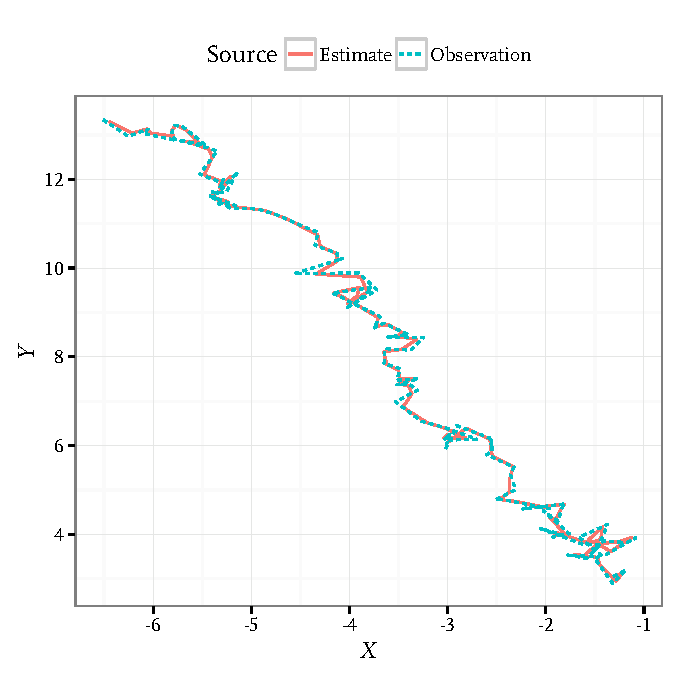
\includegraphics{fig/pf}
  \caption{Estimates and observations of the particle filter}
  \label{fig:pf}
\end{figure}
